\documentclass[abstract=on,10pt,a4paper,bibliography=totocnumbered]{article}
\usepackage[paper=a4paper,left=35mm,right=35mm,top=25mm,bottom=30mm]{geometry}
\usepackage[doublespacing]{setspace}
\usepackage[english]{babel}
\usepackage[utf8]{inputenc}
\usepackage[round]{natbib}
\usepackage{amsmath}
\usepackage{colortbl}
\usepackage{amsfonts}
\usepackage{amssymb}
\usepackage{gensymb}
\usepackage{graphicx}
\usepackage{tikz}
\usepackage{enumerate}
\usepackage{enumitem}
\usepackage{subcaption}
\usepackage{booktabs}
\usepackage[hidelinks]{hyperref}
\usepackage[nameinlink]{cleveref}
\usepackage{lineno}
\usepackage{multirow}
\usepackage{arydshln}
\usepackage[nomarkers, nolists]{endfloat}

%------------------------------------------------------------------------------
%	Some Styling
%------------------------------------------------------------------------------
% Creating some TikZ styles
\tikzset{
  nonterminal/.style = {rectangle
    , minimum size = 6mm
    , very thick
    , draw = black!
  }
}

% Changing the style of captions in figures etc.
\captionsetup{labelfont=bf, format=plain, font=small}

%------------------------------------------------------------------------------
%	Titlepage: Header
%------------------------------------------------------------------------------
\title{Bound within Boundaries? How Well Do Boundaries of Protected Areas Match
Movement Corridors of Their Most Mobile Protected Species?}

% List of Authors
\author{
  David Hofmann\textsuperscript{1\S} \and
  John W. McNutt\textsuperscript{2} \and
  Arpat Ozgul\textsuperscript{1} \and
  Dominik Behr\textsuperscript{1,2*} \and
  Gabriele Cozzi\textsuperscript{1,2*} \and
}

% Reduce spacing between authors
\makeatletter
\def\and{%
  \end{tabular}%
  \hskip -0.5em \@plus.17fil\relax
  \begin{tabular}[t]{c}}
\makeatother

% Current Date
\date{\today}

% And here the masterpiece begins
\begin{document}

% Change page numbering
\pagenumbering{gobble}

% Required to be able to cite
\bibliographystyle{apalike}

% Create Titlepage
\maketitle

%------------------------------------------------------------------------------
%	Titlepage: Additional Info
%------------------------------------------------------------------------------
\begin{flushleft}

\vspace{0.5cm}

\textsuperscript{1} Department of Evolutionary Biology and Environmental
Studies, University of Zurich, Winterthurerstarsse 190, 8057 Zurich,
Switzerland.

\textsuperscript{2} Botswana Predator Conservation Trust, Private Bag 13, Maun,
Botswana.

\textsuperscript{\S} Corresponding author (david.hofmann2@uzh.ch)

\textsuperscript{*} Shared senior co-authorship

\vspace{4cm}

\textbf{Running Title:} Connectivity across a Transfrontier Conservation Area.

\vspace{0.5cm}

\textbf{Keywords:} Lycaon pictus, KAZA-TFCA, permeability surface, least-cost
corridors, integrated step selection function, landscape connectivity

\end{flushleft}

%------------------------------------------------------------------------------
%	Abstract
%------------------------------------------------------------------------------
\newpage
\begin{abstract}
\noindent In response to the global deterioration and fragmentation of suitable
habitats, large portions of land have been set aside to maintain and restore
connectivity among wildlife subpopulations. While boundaries of such
conservation areas are often based on expert opinion and socio-political needs
and constraints, the extent to which their boundaries match movement corridors
of their protected species is rarely assessed. This is mainly due to lack of
adequate data. One such conservation area is the Kavango-Zambezi Transfrontier
Conservation Area (KAZA-TFCA) in Africa, which, spanning five countries and
520'000 km\textsuperscript{2}, is the largest transboundary conservation area in
the world.

\noindent Between 2011 and 2019, we collected novel high-resolution GPS
relocation data on dispersing African wild dogs (\textit{Lycaon pictus}) to
assess to which degree the KAZA-TFCA boundaries reflect natural movement
corridors of this highly mobile and critically endangered species.

\noindent We demonstrate that the major dispersal corridors were within the broad
KAZA-TFCA boundaries, yet some run outside formally-protected areas. Further, we
identified significant differences in permeability to movement across the five
KAZA-TFCA countries. Such differences were mainly due to different degrees of
human activities, which hampered dispersal movements.

\noindent Our work shows the importance of empirically assessing the adequacy of
protected areas boundaries and the need for international coordination that stem
from different contribution to connectivity
\end{abstract}

%------------------------------------------------------------------------------
%	Main Text
%------------------------------------------------------------------------------
\newpage

% Change page numbering
\pagenumbering{arabic}

% Create linenumbers
\linenumbers

\section{Introduction}
As a result of the ongoing human-caused habitat deterioration and fragmentation,
successful management and conservation of isolated subpopulations requires
maintenance and enhancement of connectivity between them \citep{Hanski.1998,
Fahrig.2003, Lindenmayer.2013}. Recently, efforts have been made to facilitate
animal movements and dispersal, and to secure connectivity by protecting
contiguous natural or semi-natural areas \citep{Heller.2009, Doerr.2011,
Rudnick.2012, Cozzi.2020}. These efforts have resulted in the creation of an
ever growing number of large and often transboundary protected areas
\citep{Wolmer.2003}, whose boundaries have been drawn based largely on expert
opinions or political reasons, often revealing deficiencies
\citep{Pullinger.2010}. Due to the very nature of such vast protected areas,
which sometimes span several thousands of square kilometers and traverse
multiple countries, a thorough assessment of their effectiveness and adequacy of
their boundaries is indeed challenging \citep{Rudnick.2012}. This challenge is
complicated by a lack of movement data at the appropriate spatial scale and an
insufficient understanding of the ranging behavior, movement patterns, and
dispersal corridors of the species for which these protected areas have been
created \citep{Vasudev.2015, Tshipa.2017, Cozzi.2020}. An accurate
representation of dispersal corridors and migratory routes based on empirical
global positioning system (GPS) data is thus fundamental to assess how well
boundaries of protected areas reflect actual animal movements \citep{Beier.2008,
Doerr.2011, Rudnick.2012}.

In recent years, there has been a growing body of research that uses animal
relocation data to identify dispersal corridors and assess connectivity at large
scales \citep{Chetkiewicz.2006, Doerr.2011, Squires.2013, Elliot.2014,
Benz.2016, Osipova.2019}. Identification of potential corridors relies on the
estimation of permeability (respectively resistance) surfaces, which return the
ease or willingness at which the focal species traverses a specific landscape
\citep{Sawyer.2011}. Such surfaces are created on the basis of habitat
preferences, which can be estimated using a suite of selections functions,
including resource selection functions \citep{Boyce.2002}, step selection
functions \citep{Fortin.2005}, and path selection functions
\citep{Cushman.2010}. These approaches have in common that they infer habitat
preferences by comparing landscape covariates (e.g. environmental and
anthropogenic) at locations visited by the animal to the same spatial covariates
at randomly selected locations \citep{Zeller.2012}. As such, these approaches
require adequate landscape and GPS relocation data that is representative of the
process being studied \citep{Diniz.2020}. More specifically, GPS relocation
data collected on dispersing individuals has been shown to outperform GPS
relocation data collected on resident individuals when the aim is to detect
large scale dispersal corridors \citep{Elliot.2014, Diniz.2020}. Few studies
have, however, partitioned their GPS relocation data according to behavioral
modes (e.g. resident vs dispersing) of the studied species \citep{Wilson.2012,
Vasudev.2015}. As such, most permeability surfaces upon which dispersal
corridors are identified are created using GPS relocation data that was
collected on resident individuals. This introduces severe biases and
substantially reduces the power to reveal meaningful movement corridors - for
dispersing individuals have different needs and motivations compared to resident
individuals \citep{Killeen.2014, Elliot.2014, Cozzi.2020} - thus limiting our
ability to assess the adequacy of the boundaries of protected areas.

One initiative that aims at restoring and enhancing connectivity across large
scales is the Kavango-Zambezi Transfrontier Conservation Area (KAZA-TFCA), which
spanning over 520'000 km\textsuperscript{2} and five countries constitutes the
largest transfrontier conservation area in the world. While the KAZA-TFCA was
originally set to facilitate movements of African elephants (\textit{Loxodonta
africana}; \citealp{Tshipa.2017}), it is also key to the conservation of  other
wide-ranging species, such as African wild dogs (\textit{Lycaon pictus};
\citealp{Woodroffe.2012, Cozzi.2020}), lions (\textit{Panthera leo};
\citealp{Elliot.2014, Cushman.2018}), and cheetahs (\textit{Acinonyx jubatus};
\citealp{Weise.2017}). To date, however, few studies have attempted to assess
the appropriateness of KAZA's boundaries using relevant GPS movement  data at
the appropriate spatial scale \citep{Elliot.2014, Tshipa.2017}. Thus, how well
the KAZA-TFCA's boundaries reflect natural movement patterns and dispersal
corridors of its protected species is virtually unknown.

A highly endangered flagship species for conservation efforts across the
KAZA-TFCA, but for which systematic GPS relocation data on dispersing
individuals is unavailable, is the African wild dog (\textit{Lycaon pictus}).
While once widespread across the entire Sub-Saharan continent, the species has
been widely extirpated through human persecution, habitat destruction, and
disease outbreaks \citep{Woodroffe.2012}. As a result, the African wild dog has
become one of Africa's most endangered large carnivores, and it currently only
survives in small, spatially scattered subpopulations \citep{Woodroffe.2012}.
Within these subpopulations, wild dogs form cooperative breeding packs of up to
thirty individuals \citep{Frame.1979, Fuller.1992, Creel.2002}. Males and
females typically disperse from their natal pack, either alone or in same-sex
dispersing coalitions, and search for unrelated mates and a suitable territory
to settle \citep{McNutt.1996, Behr.2020}. During dispersal, wild dogs can cover
several hundred kilometers, sometimes crossing national boundaries and areas
strongly influenced by humans \citep{DaviesMostert.2012, Masenga.2016,
Cozzi.2020}. To date, little empirical information is available on habitat
selection and movement behavior of wild dogs during dispersal. The few studies
that have collected GPS relocation data during dispersal have demonstrated that
dispersers generally avoid human-dominated landscapes \citep{Masenga.2016,
Oneill.2020, Cozzi.2020} and areas densely forested \citep{Oneill.2020},
whereas they prefer proximity to water and dust roads \citep{Oneill.2020}.

Here, we used GPS relocation data collected on 16 wild dogs in as many
dispersing coalitions from a free-ranging population to assess the adequacy of
the boundaries of the KAZA-TFCA, the largest protected area in the world. To
this end, we estimated the degree of selection or avoidance for environmental
and anthropogenic landscape features and used the obtained information to create
a permeability surface.  This allowed us to investigate how landscape
permeability varies regionally and internationally and to identify major
dispersal corridors and dispersal hubs.

\section{Methods}
\subsection{Study Area}
The study area (centered at -17\degree 13'9''S, 23\degree 56'4''E; elevation ca.
1'030 m, red rectangle in \Cref{StudyArea} was confined by a bounding box
encompassing the entire KAZA-TFCA. was outlined by a rectangular bounding box
stretching over 1.3 Mio km\textsuperscript{2} and encompassing the entire
KAZA-TFCA. The KAZA-TFCA lies in the basins of the Okavango and Zambezi rivers
and includes parts of Angola, Botswana, Namibia, Zimbabwe, and Zambia. With a
total area of over 520'000 km\textsuperscript{2} it covers several
already-existing national parks (NPs) and other protected areas. It constitutes
the earth's largest transboundary conservation area and is characterized by
diverse landscapes, including savanna, grassland, and dry or moist woodland
habitats. Rainfall in the study area is seasonal and lasts from November to
March, whereas the rest of the year remains dry \citep{McNutt.1996,
Mendelsohn.2010}. The KAZA-TFCA also encloses the Okavango Delta, which is one
of the main strongholds of African wild dogs in southern Africa and likely acts
as a source for the recolonization of surrounding habitats
\citep{Woodroffe.2012, Cozzi.2013}. The extent of the flood in the delta greatly
changes within and between years depending on the amount of rain that descends
from the catchment areas in Angola and reaches the distal ends of the delta
between July and August (Figure XX in Appendix XX for an illustration of a
typical flood pulse). The flood drastically affects surrounding landscapes, so
that during maximum extent (ca. 12'000 km\textsuperscript{2}) the delta becomes
a patchy conglomerate of swamps, open water, and islands, whereas these
structures disappear when the flood retracts (ca. 5'000 km\textsuperscript{2})
during dry periods \citep{Gumbricht.2004, Wolski.2017}. Despite 36 NPs and other
protected areas, there is considerable human influence in some regions of the
KAZA-TFCA, mainly originating from human activities on farms, high human
density, and road traffic.

\begin{figure}[h]
  \begin{center}
    \begin{tikzpicture}
        \node[anchor=south west,inner sep=0] (image) at (0,0,0) {
        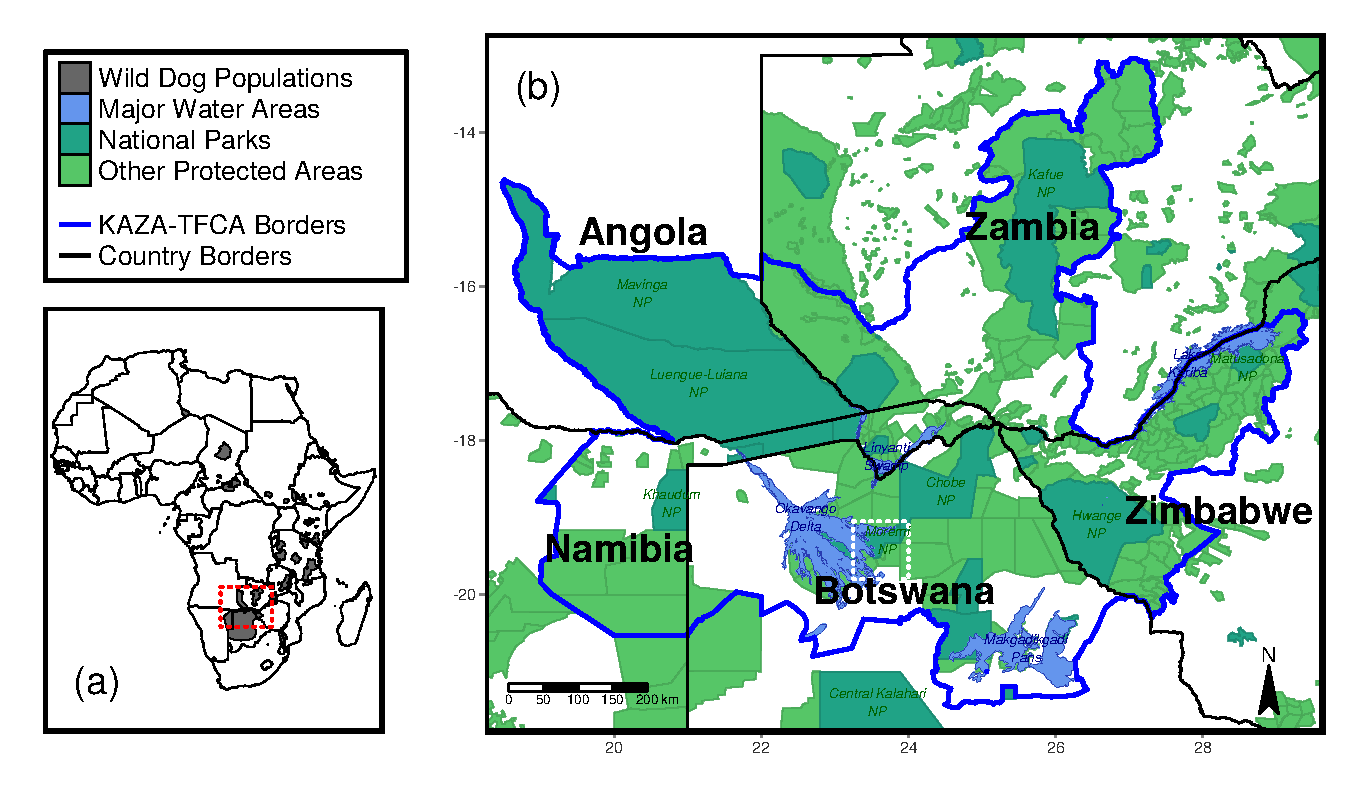
\includegraphics[width=\textwidth]{99_StudyArea.pdf}
        };
        \begin{scope}[x={(image.south east)},y={(image.north west)}]
            % % next four lines will help you to locate the point needed by forming a grid.
            % % comment these four lines in the final picture.
            % \draw[help lines,xstep=.1,ystep=.1] (0,0) grid (1,1);
            % \draw[help lines,xstep=.05,ystep=.05] (0,0) grid (1,1);
            % \foreach \x in {0,1,...,9} { \node [anchor=north] at (\x/10,0) {0.\x}; }
            % \foreach \y in {0,1,...,9} { \node [anchor=east] at (0,\y/10) {0.\y};}
            % % upto here
            \draw[black] (0.202, 0.255) -- (0.36, 0.955);
            \draw[black] (0.202, 0.205) -- (0.36, 0.070);
        \end{scope}
    \end{tikzpicture}
    \caption{Overview of our study area. (a) The red rectangle depicts the study
    area, which was confined by a bounding box encompassing the entire
    KAZA-TFCA. Pink areas indicate remaining wild dog populations according to
    the IUCN \citep{Woodroffe.2012}. (b) The white rectangle illustrates the
    area within which dispersal coalitions were collared. Since Game Reserves in
    Botswana virtually serve the same purpose as National Parks, we use the
    terms interchangeably for this region.}
    \label{StudyArea}
  \end{center}
\end{figure}


\subsection{GPS Relocation Data}
We used a population of free-ranging African wild dogs inhabiting the Okavango
Delta in northern Botswana as a source population for dispersing individuals.
This population has been extensively studied since 1989 \citep{McNutt.1996,
McNutt.2008, Cozzi.2013, Cozzi.2020, Behr.2020}. We collected GPS relocation
data of 16 wild dog coalitions (7 female and 9 male coalitions) that dispersed
between 2011 and 2019 (see also \citealp{Abrahms.2017} and
\citealp{Cozzi.2020}). Candidate dispersing individuals were identified based on
procedures reported in \cite{Behr.2020}, immobilized according to protocols
described in \cite{Osofsky.1996}, and fitted with GPS/Satellite radio collars
(\textit{Vertex Lite; Vectronic Aerospace GmbH, Berlin}) while still in their
natal pack. All required procedures were undertaken and supervised by a
Botswana-registered wildlife veterinarian. Immobilized individuals were
monitored and all were observed to successfully re-join their packs within one
hour after immobilization. During dispersal, GPS collars were programmed to
record GPS relocation data every 4 hours and to regularly transmit them via
Iridium satellite system to a base station. The system thus allowed
remote-tracking of collared individuals, even where field conditions were
prohibitive or dispersal trajectories crossed international borders.

Because we were interested in recording dispersal trajectories, we discarded any
GPS data collected while individuals were still with their natal packs
\citep{Cozzi.2020}. Dispersal periods were identified based on supporting
information from the field, as well as from plotting and visually inspecting the
net squared displacement (NSD) metric for each dispersing coalition. NSD is a
metric indicating the euclidean distance of a relocation to a reference point
\citep{Borger.2012}, which in our case was the center of the dispersing
coalition's natal home range. Thus, dispersal was deemed to have started when a
coalition had left its natal home range and continued until the NSD metric
remained stationary, implying that the coalition settled (Figure XX in Appendix
XX). Some coalitions undertook exploratory movements prior to proper dispersal.
Such movements have been observed in other species and are reported to be very
similar to proper dispersal \citep{Killeen.2014}, so we classified exploratory
movements as dispersal too. In total, we collected 4'169 GPS relocations during
dispersal (Figure XX and Table XX in Appendix XX) for an average of 260
locations/coalition (range: 37 - 729). On average, dispersing coalitions
dispersed for 48 days (min = 9, max = 137), covered a mean euclidean distance of
54 km (min = 3, max = 263) and a mean cumulative distance of 596 km (min = 130,
max = 1'962). In our analysis, we did not differentiate between male and female
dispersing coalitions, for previous research found little differences between
sexes during dispersal \citep{Woodroffe.2019, Cozzi.2020}.

\subsection{Spatial Covariates}
We used a set of geo-referenced covariates to investigate habitat preferences of
dispersing wild dogs (\Cref{Covariates}). Covariates fell into the categories
\textit{land cover}, \textit{protection status}, and \textit{human influence}.
Due to the absence of noteworthy elevational gradients in our study area we did
not include terrain features as covariates. For each covariate, we prepared
spatial raster layers from freely available online services or from remotely
sensed satellite imagery. To ensure a consistent resolution (i.e. cell-size or
grain) across covariates, we coarsened or interpolated all layers to match a
resolution of 250m x 250m. We performed processing and manipulation of data, as
well as all spatial and statistical analyses, using R, version 3.6.1
\citep{R.2019}).

\begin{figure}[h]
  \begin{center}
    \includegraphics[width = \textwidth]{99_Covariates.pdf}
    \caption{Overview of spatial covariates that we included in our models. We
    prepared all covariates for the entire study area but for better visibility
    we only plot them for the surroundings of the Okavango Delta. The white
    rectangle in each plot depicts the area within which dispersal coalitions
    were collared. (a) Averaged layer of all dynamic (binary) watermaps. (b)
    Percentage cover of trees. (c) Percentage cover of shrubs/grassland.
    Anything that was not covered by trees or shrubs/grassland was deemed to be
    bare land. (d) Protection status of the area. (e) Human influence proxy
    composed of human density, farms, and roads. (f) Distance to nearest road
    (white lines depict actual roads).}
    \label{Covariates}
  \end{center}
\end{figure}

\subsubsection{Land Cover}
We divided land cover into water (1) and dryland (2), and we further subdivided
dryland into three categories.

\begin{enumerate}[label = (\arabic*)]

  \item Water included rivers, wetlands, and swamps. Because the
  inundation extent of the flood in the Okavango Delta is highly variable within
  and between years, we created weekly (8 daily)  ``floodmaps'' , following a
  remote sensing algorithm developed by \citep{Wolski.2017}. The algorithm uses
  thresholding of short wavelength infrared reflectances of MODIS Terra
  satellite imagery (MCD43A4, \citealp{Schaaf.2015}) to distinguish areas
  covered by water and dryland (details in Appendix XX). While we created
  dynamic floodmaps for the Okavango Delta, we assumed all other water bodies
  (e.g. Chobe river, Zambezi river) to be static within and between years. This
  static representation was based on Globeland's land cover dataset
  \citep{Chen.2015}, from which we only retained the categories \textit{wetland}
  and \textit{water bodies} and collectively reclassified them to
  \textit{water}. Globeland had an original resolution of 30m x 30m, so we
  coarsened the layer to 250m x 250m using the mode of each 250m x 250m cell. We
  further improved river representation using the rasterized MERIT Hydro dataset
  \citep{Yamazaki.2019}, from which which we added all rivers with a width of
  over 10m to our Globeland layer. Finally, we merged dynamic and static
  watermaps into a large rasterstack, covering the entire study area.

  \item We subdivided dryland into three categories as derived from the
  MODIS Terra Vegetation Continuous Fields dataset (MOD44B,
  \citealp{Dimiceli.2015}). Combined, the three layers added up to 100\% and
  depicted the percentage cover of tree-vegetation (henceforth trees),
  non-tree-vegetation (henceforth shrubs/grassland), and non-vegetated
  (henceforth bare land).  We used our floodmap that aligned with the creation
  date of these MODIS layers (30 March 2017) and defined anything covered by
  water as 0\% vegetated. The MODIS vegetation layers had a resolution of 250m x
  250m, so we did not need to coarsen or interpolate them.

\end{enumerate}

\subsubsection{Proection Status}
We created a binary layer separating protected from unprotected land. We
downloaded corresponding data on protection status from the Peace Parks
Foundation (\url{www.peaceparks.org}; \citealp{PeaceParks.2019}). Protected
areas included forest reserves, game reserves, wildlife management areas, and
national parks. We classified anything not covered by these categories as
unprotected (e.g. communal pastoral land, private land). We rasterized the two
categories onto a binary raster (1 = protected, 0 = pastoral) with a resolution
of 250m x 250m.

\subsubsection{Human Influence}
We created a layer representing human influence by integrating information on
(1) human density, (2) farming activities, and (3) roads.

\begin{enumerate}[label = (\arabic*)]

  \item We obtained spatial human density estimates through Facebook's 30m x 30m
  high-resolution population density dataset (\url{www.dataforgood.fb.com};
  \citealp{Facebook.2019}). The layer was coarsened to 250m x 250m by summing up
  human density values within each 250m x 250m cell.

  \item We sourced Information on farming activities from the Globeland
  \citep{Chen.2015} and Cropland \citep{Xiong.2017} land cover datasets, from
  which we retained areas that were classified as either \textit{cultivated
  land} or \textit{croplands}. Any other land cover classes were not pertinent
  to farming and therefore omitted. Because both layers had a resolution of 30m
  x 30m we coarsened them to 250m x 250m by assigning a value of 1 to any 250m x
  250m cell that covered farmland and a value 0 otherwise. Thus the final layer
  depicted presence (= 1) or absence (= 0) of farms within each 250m x 250m
  cell.

  \item We obtained geo-referenced data on roads from Open Street Map through
  Geofabrik (\url{www.geofabrik.de}; \citealp{Geofabrik.2019}). We only retained
  main tar roads and omitted smaller roads (see Table XX in Appendix XX) as
  these are scarcely frequented and do not represent an obstacle to dog
  movements \citep{Abrahms.2016}. Finally, we rasterized roads to a binary
  raster (1 = roads, 0 = no roads) with 250m x 250m resolution.

\end{enumerate}

\noindent To calculate a single proxy of human influence, we added up the layers
describing human density (continuous), farming (binary), and roads (binary). To
reduce the influence of outliers, totaled values were limited to a maximum of
50, which visually resulted in a good balance between high and low anthropogenic
influence and was therefore considered appropriate for our analysis. To render
the fact that humans influence their surroundings beyond their presence, we
followed \cite{Elliot.2014} and applied to each cell a 5 km spatial buffer
within which we summed up and log-transformed human-influence values (Figure XX
in Appendix XX).

\subsection{Habitat Selection Model}
We used an integrated step selection function (iSSF, \citealp{Avgar.2016}) to
investigate dispersers' selection or avoidance for the above mentioned spatial
covariates. In the iSSF framework, GPS relocations are coerced to  ``steps'',
where a step is defined as the connecting line between two consecutive GPS
relocations \citep{Turchin.1998}. Subsequently, habitat preferences are
estimated by contrasting covariates along realized steps to the same covariates
along alternative ``random''  steps \citep{Fortin.2005, Thurfjell.2014,
Avgar.2016}. Thus, we paired each realized step with 24 random steps. We
generated random steps by sampling turning angles from a uniform distribution
U(\(-\pi, \pi\)) and step lengths from a gamma distribution that was fitted
using realized steps \citep{Avgar.2016}. Together, a realized and its 24
associated random steps formed a stratum of 25 steps that received a unique
identifier. We extracted covariates along all steps (Table XX in Appendix XX),
standardized them using a z-score transformation, and checked for correlation
using Pearson's Correlation Coefficient. None of the covariates were overly
correlated (\(|r| > 0.6\), \citealp{Latham.2011}) and we retained all of them
for modeling. Our habitat selection was then based on the assumption that
dispersing wild dogs assigned a selection score \(w(x)\) of the following
exponential form to each realized and random step:

\begin{equation}
\label{EQ1}
  w(x) = exp(\beta_1 x_1 + \beta_2 x_2 + ... + \beta_n x_n)
\end{equation}

\noindent The selection score \(w(x)\) of a step depended on its associated
covariates (\(x_1, x_2, ..., x_n\)), as well as on the animal's preferences for
these covariates (\(\beta_1, \beta_2, ..., \beta_n\)). To estimate habitat
preferences (i.e. the \(\beta\)'s) of interest, we used mixed effects
conditional logistic regression analysis as suggested by \cite{Muff.2019}. We
implemented their method using the R-package \textit{glmmTMB}
\citep{Mollie.2017} and used coalition ID to model random intercepts and slopes.
We defined two movement metrics, namely the cosine of the turning angle
(\(cos(ta)\)) and the log of the step length (\(log(sl)\)), as core covariates
and ran stepwise forward model selection based on Akaike's Information Criterion
(AIC, \citealp{Burnham.2002}) for all other covariates. The inclusion of the
movement metrics served to reduce biases in estimated habitat preferences that
may have arised due to movement preferences \citep{Avgar.2016}.

To validate the predictive power of the most parsimonious habitat selection
model, we ran k-fold cross-validation for case-control studies as described in
\cite{Fortin.2009}. This procedure compares rank frequencies of realized steps
under observed and random preferences and proofs a significant prediction in
case the confidence intervals of the spearman-rank correlation coefficients
\(\bar{r}_{s, realized}\) and \(\bar{r}_{s, random}\) do not overlap (Appendix
XX).

\subsection{Permeability Surface}
Using the most parsimonious selection model, we predicted a permeability surface
spanning the entire extent of the KAZA-TFCA. That is, we applied \Cref{EQ1} to
our spatial covariates and calculated the selection score \(w(x)\) for each
raster-cell in our study area. To reduce the influence of outliers in predicted
scores, we followed \cite{Squires.2013} and curtailed predicted scores between
the 1\textsuperscript{st} and 99\textsuperscript{th} percentile of their
original values. Because our floodmaps were dynamic, we collapsed all floodmaps
into a single static layer using areas that were covered by water in at least a
quarter of all our floodmaps. To compare permeability across different regions,
we rescaled the permeability surface to a range between 0 and 1. The most
impermeable landscape thus received a value of 0, the most permeable landscape a
value of 1.

\subsection{Least-Cost Paths \& Least-Cost Corridors}
To identify movement corridors within the extent of the KAZA-TFCA, we specified
source points and calculated factorial least-cost paths (LCPs), as well as
factorial least-cost corridors (LCCs), between them (Figure XX in Appendix XX;
\citealp{Adriaensen.2003, Sawyer.2011, Elliot.2014}. We generated source points
by overlaying the study area with a regular grid of points spaced at 100 km. We
only considered those points that fell within protected areas \(>\) 700
km\textsuperscript{2}, which conforms with home-range requirements of African
wild dogs reported in \cite{Pomilia.2015}. Finally, we defined centroids as
source points for those protected areas \(>\) 700 km\textsuperscript{2} that
were not assigned any source points from the regular grid. In total, we
generated 68 source points, which resulted in 2'278 unique pairwise combinations
and therefore 2'278 unique LCPs and LCCs.

We implemented factorial LCP analysis between source points using the R-package
\textit{gdistance} (Figure XX in Appendix XX, \citealp{vanEtten.2018}). The
package translated the (unscaled) permeability surface into a network of nodes
to find shortest effective distances between source points based on
probabilities of moving from cell to cell. In our case, the transition
probability of moving between two adjacent cells depended on their averaged
permeability. We allowed individuals to move from each cell to the cell's 8
surrounding neighbors (i.e. Moores neighborhood) and applied a geographic
correction to account for the fact that diagonal neighbors were more remote than
orthogonal neighbors. Because African wild dogs have been observed to cover
large dispersal distances \cite{DaviesMostert.2012, Masenga.2016, Cozzi.2020},
we did not limit LCPs to a maximal effective cost. After computation, we tallied
overlapping LCPs and identified high-frequency routes.

We calculated factorial LCCs \cite{Pinto.2009, Sawyer.2011, Elliot.2014}, again
using the R-package gdistance (Figure XX in Appendix XX,
\citealp{vanEtten.2018}). To identify LCCs, we first computed for each source
point a cumulative cost map, which indicated the total minimal costs required to
get from the source point to any other cell in the study area. An LCC between
two points was then obtained by adding up their cumulative cost maps and masking
out all cell-values exceeding the lowest cell-value by more than 5\%
\citep{Pinto.2009}. We repeated this procedure for each possible unique pairwise
combination of source points and thereby identified LCCs between all 68 selected
points. We normalized the resulting corridor-maps to range from zero to one and
merged them into a single connectivity map.

\section{Results}
\subsection{Habitat Selection Model}
Our most parsimonious habitat selection model (\(\Delta AIC > 2\) than any
alternative model; Table XX in Appendix XX) retained the covariates
\textit{Water}, \textit{DistanceToWater}, \textit{Trees},
\textit{Shrubs/Grassland}, and \textit{HumansBuff5000}, beside the fixed
covariates \textit{cos(ta)} and \textit{log(sl)} (\Cref{PermeabilityResults}a).
Parameter estimates showed that dispersing wild dogs moved in a directional and
fast manner, as indicated by a positive selection for small turning angles, i.e.
high \(cos(ta)\) (\(\beta\) = 0.14; 95\% CI = 0.07 to 0.21,
\Cref{PermeabilityResults}a) and longer steps, i.e. high \(log(sl)\) (\(\beta\)
= 0.05, 95\% CI = 0.02 to 0.09, \Cref{PermeabilityResults}a). Dispersers avoided
moving through open water (\(\beta\) = -0.49, 95\% CI -0.67 to -0.30) but
selected for locations in its vicinity, although the latter effect was not
significant (\(\beta\) = -0.31, 95\% CI = -0.70 to 0.09,
\Cref{PermeabilityResults}a). Dispersers avoided areas that were densely covered
by trees (\(\beta\) = -0.17, CI = -0.33 to -0.01, \Cref{PermeabilityResults}a)
and preferred areas covered by shrubs/grassland (\(\beta\) = 0.44, 95\% CI =
0.30 to 0.58, \Cref{PermeabilityResults}a). Finally, dispersers avoided areas
that were influenced by human presence and activities (\(\beta\) = -0.41, 95\%
CI = -0.78 to -0.05, \Cref{PermeabilityResults}a).

\begin{figure}[h]
  \begin{center}
    \includegraphics[width = \textwidth]{99_PermeabilityResults.pdf}
    \caption{(a) Estimated selection coefficients from the most parsimonious
    habitat selection model. Negative coefficients indicate avoidance of a
    covariate, positive coefficients selection of a covariate. Whiskers
    delineate the 95\%-CIs for estimated parameters. (b) Results from the k-fold
    cross validation for case-control studies. The left graph shows rank
    frequencies of \textit{realized} steps according to predictions, whereas the
    right graph shows rank frequencies of \textit{randomly selected} steps
    according to predictions. \(\bar{r}_s\) indicates the mean correlation
    coefficient resulting from 100 repetitions of the k-fold cross validation.
    The blue smoothing line was fitted using a locally weighted polynomial
    regression and serves to aid the eye in detecting the trends. Correlation
    coefficients suggest that our prediction was significant and robust,
    evidenced by the fact that the confidence intervals of \(\bar{r}_{s,
    realized}\) and \(\bar{r}_{s, random}\) did overlap and by the fact that
    there was strong and significant correlation between ranks and associated
    frequency for realized steps.}
    \label{PermeabilityResults}
  \end{center}
\end{figure}

Results from the k-fold cross-validation suggested that our prediction was
significant and robust, as highlighted by the fact that the 95\%-CIs intervals
of \(\bar{r}_{s, realized}\) and \(\bar{r}_{s, random}\) (0.04, CI = 0.01 to
0.08) did not overlap (\Cref{PermeabilityResults}b). Likewise, the significant
correlation between ranks and corresponding frequencies for realized steps
suggested a good fit between predictions and observations.

\subsection{Permeability Surface}
Our prediction of landscape permeability revealed substantial differences across
regions in the study area (\Cref{PermeabilityMap}). Comparisons of median
permeability values (\Cref{PermeabilityComp}) showed that permeability inside
the boundaries of the KAZA-TFCA was more than two times as high as permeability
outside it. A comparison across countries showed that Angola and Botswana were
characterized by comparably highly permeable landscapes, Zimbabwe and Zambia
were relatively impermeable, and Namibia ranged in between the two extremes
(\Cref{PermeabilityComp}). Visual inspection of our covariate layers indicated
that high permeability in Botswana and Angola is mainly caused by a combination
of low human presence and activities, low tree cover, high shrubs/grassland
cover, and a close distance to water. Although swamps, wetlands, and permanent
water themselves provide little permeability, their surroundings act as strong
attractants to dispersers. The low permeability that characterizes Zambia and
Zimbabwe, on the other hand, is mainly caused by severe anthropogenic presence
and other human activities. Albeit the KAZA-TFCA covers a majority of
permeability hot-spots, several highly permeable regions remain uncovered by its
borders, offering exciting opportunities for future expansions of already
existing protected areas. Across all countries, protected areas provided higher
permeability than human-dominated landscapes. A visual assessment of our
permeability surface futhermore revealed that northern Botswana had the highest
density of permeable landscapes (\Cref{PermeabilityMap}, bright yellow colors),
although the waters of the Okavango Delta and Linyanti Swamp themselves provided
highly impermeable landscapes (\Cref{PermeabilityMap}, dark blue colors).

\begin{figure}[hbtp]
  \begin{center}
    \begin{tikzpicture}
        \node[anchor=south west,inner sep=0] (image) at (0,0,0) {
          \begin{minipage}{\textwidth}
            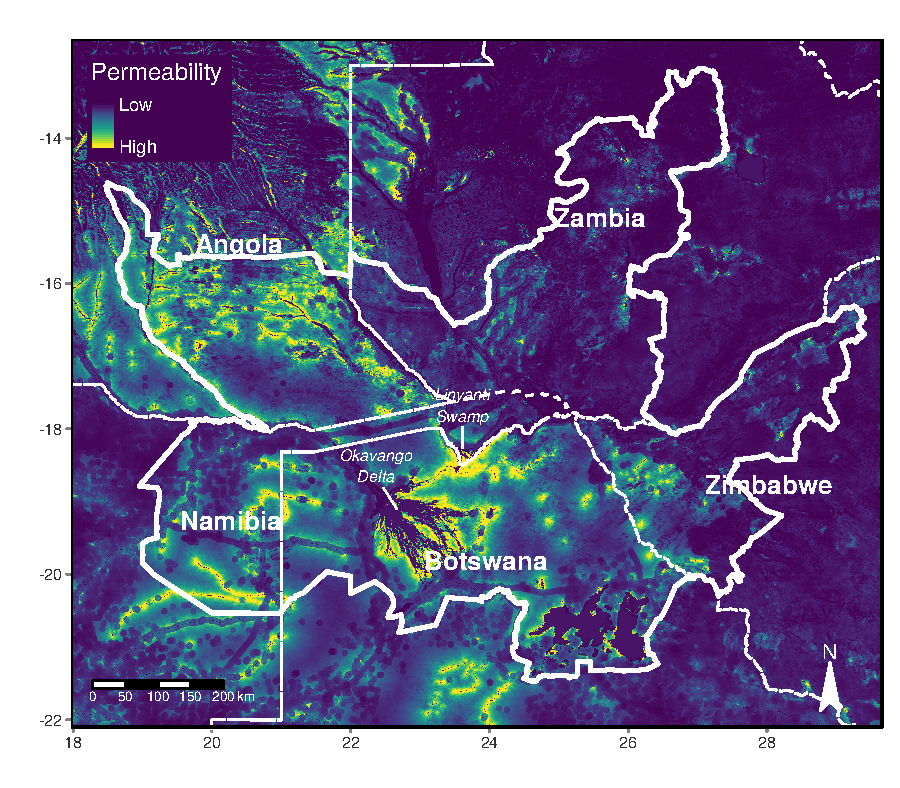
\includegraphics[width = \textwidth]{99_PermeabilityMap.pdf}
          \end{minipage}
        };
        \begin{scope}[x={(image.south east)},y={(image.north west)}]
        \end{scope}
    \end{tikzpicture}
    \caption{Predicted permeability surface for the extent of the KAZA-TFCA.
    Permability was predicted by calculating selection scores \(w(x) =
    exp(\beta_1 x_1 + \beta_2 x_2 + ... + \beta_n x_n)\) for each pixel based on
    the pixel's underlying covariates (\(x_i\)) and estimated habitat
    preferences (\(\beta_i\)). Areas that dispersers find easy to traverse are
    depicted in bright colors. Bold white lines delineate the borders of the
    KAZA-TFCA, whereas dashed white lines show country borders.}
    \label{PermeabilityMap}
  \end{center}
\end{figure}

\begin{table}[h]
  \begin{center}
  \caption{Comparison of median permeability (interquantile range in brackets)
  across countries, separated according to areas within and outside the
  KAZA-TFCA, as well as within and outside formally protected areas. High values
  indicate high permeability, whereas low values correspond to low
  permeability.}
  \label{PermeabilityComp}
  \begin{tabular}{llllll}
    \toprule
    \multicolumn{1}{c}{ } & \multicolumn{2}{c}{KAZA-TFCA} & \multicolumn{2}{c}{Protection Status} & \multicolumn{1}{c}{ } \\
    \cmidrule(l{3pt}r{3pt}){2-3} \cmidrule(l{3pt}r{3pt}){4-5}
    Country & Inside & Outside & Protected & Pastoral & Overall\\
    \midrule
    Angola & 0.41 (0.42) & 0.18 (0.35) & 0.41 (0.42) & 0.19 (0.35) & 0.26 (0.40) \\
    Botswana & 0.27 (0.30) & 0.15 (0.17) & 0.29 (0.35) & 0.16 (0.19) & 0.20 (0.26) \\
    Namibia & 0.23 (0.30) & 0.13 (0.18) & 0.24 (0.30) & 0.11 (0.15) & 0.16 (0.24) \\
    Zambia & 0.08 (0.11) & 0.04 (0.06) & 0.07 (0.12) & 0.04 (0.06) & 0.05 (0.08) \\
    Zimbabwe & 0.08 (0.20) & 0.06 (0.05) & 0.10 (0.21) & 0.06 (0.04) & 0.06 (0.08) \\
    \hline
    Overall & 0.19 (0.32) & 0.08 (0.16) & 0.18 (0.32) & 0.08 (0.17) & 0.11 (0.23)\\
    \bottomrule
  \end{tabular}
  \end{center}
\end{table}

\subsection{Least-Cost Paths \& Least-Cost Corridors}
Our least-cost analysis revealed three major movement corridors, all well-within
the KAZA-TFCA boundaries (\Cref{LeastCost}). Additionally, we found little to no
direct connectivity between peripheral points; that is, most paths and corridors
connecting two adjacent peripheral points run through more central regions
before heading towards their destination at the periphery (\Cref{LeastCost}).
One major corridor runs SE-NW and connects the Okavango-Linyanti ecosystem in
Botswana with Luengue-Luiana NP in Angola. One runs W-E between Chobe NP in
Botswana and Zimbabwe's Hwange NP. One runs NE-SW, completely across unprotected
areas, and connects Kafue NP in Zambia with more central regions of the
KAZA-TFCA. With 637 LCPs passing through it, the Okavango-Linyanti region is the
highest frequented corridor. Several minor routes branch off these three major
corridors; this includes a southward connection between the Okavango-Linyanti
and the Central Kalahari Game Reserve, a southwesterly corridor connecting
Luengue-Luiana NP with Namibia's Kaudom NP, and a northeasterly extension of the
Hwange corridor into Zimbabwe's Matusadona NP. Our model did not detect any
significant direct corridors between Zimbabwe and Zambia or Zambia and Angola,
and only a very limited W-E direct connection between the Okavango region and
Namibia's Khaudum NP. Except for the corridor into the Central Kalahari
National Park, our model did not detect any significant connectivity outside the
boundaries of KAZA-TFCA.

\begin{figure}[hbtp]
  \begin{center}
    \begin{minipage}{0.95\textwidth}
      \includegraphics[width = 0.95\textwidth]{99_LeastCostPaths.pdf}
      \includegraphics[width = 0.95\textwidth]{99_LeastCostCorrs.pdf}
    \end{minipage}
    \caption{(a) Source points (black dots) and corresponding least-cost paths
    leaving from protected areas (light grey). Note that only contiguous
    protected areas covering more than 700 km\textsuperscript{2} are depicted.
    Continuous thin black lines indicate the borders of the KAZA-TFCA, whereas
    dashed black lines delineate country-borders. (b) Least-cost corridors
    between the same source points as illustrated in subfigure (a). For ease of
    spatial reference we also labeled some national parks (dark-grey).}
    \label{LeastCost}
  \end{center}
\end{figure}

\section{Discussion}
We used GPS relocation data collected on dispersing African wild dogs to
investigate whether major movement corridors are contained within the boundaries
of the world's largest transboundary conservation area. Our analysis suggests
that the KAZA-TFCA indeed encompasses all major movement corridors of African
wild dogs, demonstrating the potential value of such an initiative. However, our
approach is neither limited to the African wild dog, nor to our study area. All
covariates used throughout this study are readily available on a global scale
and many of them are likely to be important determinants of movement behavior,
landscape permeability, and connectivity for other species
\citep{Thurfjell.2014, Zeller.2012}. Interestingly, our predicted network of
least cost-paths and least-cost corridors for African wild dogs shows surprising
similarities to corridors of dispersing lions inhabiting the same ecosystem
\citep{Elliot.2014}. This not only reinforces confidence in our own predictions
but also suggests potential synergies for the conservation of these two, and
possibly more, species. Expanding this analytical framework to additional
species will yield important insights on the consistency of inter-specific
movement corridors, thus highlighting areas that are exceptionally valuable for
the conservation of several species, rather than focusing on single species.

We identified movement corridors between pre-defined start and end points
selected within already existing protected areas. This implicitly assumes that
individuals know the end point of their dispersal journey and that they have
almost complete knowledge of associated movement costs, which is clearly not the
case \citep{Abrahms.2017}. However, creation of pre-defined end points might not
be necessary, as it should be possible to simulate dispersal from known
source-points, yet without restricting the domain of potential end points
\citep{Signer.2017}. As a consequence, movement corridors would emerge naturally
as the result of a myriad of simulated dispersal events. While this approach is
conceptually straightforward, it requires a comprehensive mechanistic
understanding of dispersal movements, which is conditioned on our ability to
appropriately represent the landscape through which individuals disperse. An
approach that does not require the creation of end points will also be
instrumental in identifying corridors outside formally protected areas. In
contrast to classical corridor mapping, individual-based movement simulations
would also allow to take into account movement preferences of dispersers, and to
render the temporal dimension of dispersal. The latter consideration is
particularly important in ecosystems where connectivity changes in response to
seasonal variations in the landscape \citep{Osipova.2019}.

Our findings emphasize that human presence and activities constitute some of the
main barriers to connectivity, which is in line with findings from eastern
Africa by \cite{Masenga.2016} and \cite{Oneill.2020}. These results are,
however, in contrast with findings by \citep{DaviesMostert.2012} who reported a
high willingness of dispersers to cross human-dominated landscapes throughout
South Africa. We believe that such differences are due to the unavailability of
alternative  ``natural''  routes in South Africa. We identified water as
additional major obstacle to dispersal, which aligns with earlier studies
showing that water is almost impermeable for resident packs and only
infrequently crossed by dispersing individuals \citep{Abrahms.2017, Cozzi.2020}.
An accurate and dynamic representation of water is therefore paramount, and
particularly important for flood-pulsing ecosystems such as the Okavango Delta.
While we found that dispersers avoided moving through water, we revealed a
preference for moving close to water. We speculate that high prey-availability
in proximity of water may partly explain this result \citep{Western.1975,
Bonyongo.2005}. Following the same logic, however, apex predators (e.g. lions,
spotted hyenas) and resident wild dogs may also prefer proximity to water
\citep{Valeix.2009} forcing dispersing wild dogs away from it
\citep{Ndaimani.2016} to avoid aggressive interactions \citep{Creel.1996,
Mills.1997}. We could not control for the presence or absence of apex predators
or conspecifics during dispersal as we lacked corresponding data, but these
considerations might explain why we did not find a statistically clear effect of
distance to water. Given the influence that resident conspecific, predators,
competitors, and prey can have during dispersal \citep{Cozzi.2018,
Armansin.2019} we urge collecting and incorporating their respective spatial
information into analyses of landscape connectivity and to more precisely
reconstruct dispersal corridors.

Locally, we identified the Okavango-Linyanti region as a potential dispersal hub
through which dispersers gain access to more peripheral regions of the
KAZA-TFCA. While this might partly be owed to the area's central position within
the KAZA-TFCA, it is likely also due to its unique environmental and
anthropogenic characteristics. In fact, the absence of human activities and the
presence of relatively impermeable water bodies, such as the Okavango Delta and
the Linyanti Swamp that potentially funnel dispersal movements, resulted in a
highly frequented corridor. The region is also instrumental for connecting wild
dog subpopulations in Zambia's Kafue and Zimbabwe's Hwange NPs. These
subpopulations are currently separated by the Zambezi River, forcing dispersers
to detour via northern Botswana to reach more peripheral areas. The key role of
the Okavango-Linyanti region for overall connectivity within the KATA-TFCA thus
calls for actions to secure its protection status in the future. While the
region is currently a Wildlife Management Area devoted to photographic tourism,
it has neither the status of a National Park nor that of a Game Reserve and so
potentially faces growing pressure towards exploitation of its natural resources
under the influences of an expanding human population, farming, and cropping
industry. A similar case of non-formally protected but key dispersal landscape
is represented by the area south of Kafue NP in Zambia, for which disruption of
its main and narrow dispersal corridor would result in considerable isolation of
its subpopulations.. We also revealed a potential southwards corridor between
the Okavango-Linyanti ecosystem and the Central Kalahari Game Reserve.
\cite{Elliot.2014} identified a similar corridor for dispersing lions,
suggesting that upholding and protecting a link between those ecosystems is
pivotal. Some areas through which the corridor runs are neither part of the
KAZA-TFCA nor profit from any form of protected status. In fact, human presence
and activities along the national road that longitudinally traverses this
corridor may limit realized connectivity \citep{Cozzi.2020}. In general, our
connectivity map suggests that connectivity gradually decreases towards the
borders of our study area, yet this might partly be a result of boundary effects
\citep{Koen.2010}.

Comparisons of landscape permeability across the extent of the KAZA-TFCA
revealed that northern Botswana and southern Angola provide relatively permeable
landscapes. Visual inspection of our covariate layers indicated that high
permeability in these countries is mainly caused by a combination of low human
presence and activities, low tree cover, high shrubs/grassland cover, and a
close distance to water. Although swamps, wetlands, and permanent water
themselves provide little permeability, their surroundings act as strong
attractants to dispersers. The low permeability that characterizes Zambia and
Zimbabwe, on the other hand, is mainly caused by severe anthropogenic presence
and other human activities. Albeit the KAZA-TFCA covers a majority of
permeability hot-spots, several highly permeable regions remain uncovered by its
borders, offering exciting opportunities for future expansions of already
existing protected areas.


%------------------------------------------------------------------------------
%	Gabs wanted to delete this
%------------------------------------------------------------------------------
% Because we predicted permeability and connectivity for such an extensive area,
% we were strongly limited in available and reliable land cover data. As a
% result, our representation of vegetation remained rather basic with only three
% vegetation classes (tree-cover, shrubs/grassland, bare land). Although some
% large-scale, high-resolution land cover datasets exist, such as Globeland's
% 30m \citep{Chen.2015} and the European Space Agency's and 20m \citep{ESA.2019}
% land cover datasets, we found their classifications often erroneous for our
% study area. This is presumably owed to the KAZA-TFCA's unique landscape and
% corresponding difficulties in remote sensing satellite imagery using
% traditional indices \citep{Wolski.2017}.

\section{Conclusion}
Our work showed that the majority of dispersal corridors for African wild dogs
are covered by the boundaries of the KAZA-TFCA, suggesting that the KAZA-TFCA
will significantly contribute to the long-term viability of this species.
Nevertheless, some unprotected dispersal routes do exist outside the KAZA-TFCA
and indicate opportunities for further expansions in the future. Moreover, our
connectivity network of least-cost paths and least-cost corridors highlights the
Okavango-Linyanti region as a central dispersal hub through which dispersers
gain access to more remote regions of the KAZA-TFCA. This stresses the
importance of northern Botswana for the conservation of this charismatic
species. Finally, our investigations showed that human pressures remain a severe
impediment to dispersal and therefore reduce landscape connectivity. Successful
conservation of the African wild dog is thus contingent on the willingness of
local authorities, policymakers, and land managers to preserve areas that are
largely liberated from human strains. Ultimately, our work contributes to the
growing field of connectivity literature and has important implications for the
management and conservation of the endangered African wild dog.

\section{Acknowledgements}
We thank the Ministry of Environment and Tourism of Botswana for granting
permission to conduct this research. We thank C. Botes, I. Clavadetscher, and G.
Camenisch for assisting with wild dog immobilizations. We thank Prof. J. Fieberg
for consulting on statistical aspects of this work and P. Wolski from the
Okavango Research Institute for assisting in generating dynamic flood maps. This
study was funded by Basler Stiftung für Biologische Forschung, Claraz
Foundation, Idea Wild, Jacot Foundation, National Geographic Society, Parrotia
Stiftung, Stiftung Temperatio, Wilderness Wildlife Trust Foundation,
Forschungkredit der Universität Zürich, and a Swiss National Science Foundation
Grant (31003A\_182286) to A. Ozgul.

\newpage
\begingroup
\singlespacing
\bibliography{Literatur}
\endgroup

\end{document}
